\documentclass{article} %article 文档
\usepackage{graphicx}
\usepackage{amssymb}
\usepackage{xcolor}
\usepackage{listings}
\usepackage{soul}

\title{Arrangement for DroneGo}  %文章标题
\author{Hao Li, Peisen Wang, Benjia Liu}   %作者的名称
\date{\today}       %日期
% 设置页面的环境,a4纸张大小,左右上下边距信息
\usepackage[a4paper,left=10mm,right=10mm,top=15mm,bottom=15mm]{geometry} 

\begin{document}
\maketitle

\begin{abstract}

% 在波多黎各遭受最严重的飓风袭击后,许多人受伤。高速公路被洪水堵塞并损坏。我们建立了一个模型,可以同时满足药物输送和带有旋翼无人机的道路侦察的需求。
% 我们的模型考虑了以下因素:货运集装箱的数量,无人机的类型和数量,药品的数量,每个货运集装箱的相关包装配置, 货运集装箱的确切位置以及每架无人机的时间表。
After the worst hurricane to ever hit Puerto Rico, lots of people were injured. Highways were blocked and damagedby the flood.
We establish a model to both meet the needs of medicine delivery and road reconnaissance with rotor wing drones.
Our model takes into account the following factors :  the number of cargo containers, the type and the number of drones, 
the number of medicines,  the associated packing configuration of each cargo, the exact locations of cargo containers.

% 第一, 通过对航拍图像进行二值化,形态学膨胀和特征点识别, 将图像转化成一张带有可通行区域(道路)和障碍物区域(非道路区域)的栅格地图并提取ROI(城市)。
% 通过此地图,我们将集装箱放置在靠近沿海且其飞行半径内道路面积最大的地点:分别是(18.10961, -65.81971), (18.43035, -66.03689), (18.45937, -66.74583)
First, by thresholding the aerial image, morphological dilate and feature point recognition, the image is transformed 
into a Occupancy Grid Map with passable area (road) and obstacle area (non-road area) and extract the ROI (city) in the same time.

%首先,我们依据波多黎各各医院间相距的空间距离和对药品的需求量确定了各集装箱的地理分布和对无人机的安排,其中包括了对无人机运输药品和勘察地形两种功能的分类:不能勘察地形但能够承载更多药品的单个F无人机用来运输药品给相距较近的两个医院,其余距离较远的医院选择用4个速度快的无人机B来运输药品。然后余下的45个B型无人机以各个城市为基点对周围的地形进行勘察,既保证了每个医院的药品需求量,又能够极大地提高侦察的有效性。
Second, we determined the geographic distribution of each container and the arrangement of drones based on the spatial distance between Puerto Rico's every hospital and the demand for medicines, which included the classification of two functions of drone , one is transportation Medicine drones, the other is the terrain survey drones: A single F drone that cannot survey the terrain but can carry more medicines is used to transport medicines to two hospitals that are closer to each other,which are located farther away Of hospitals were selected to use 4 fast drones B to transport medicines.Then the remaining 45 B-type UAVs surveyed the surrounding terrain with each city as the base point, which not only ensured the drug demand of each hospital, but also greatly improved the effectiveness of the reconnaissance.

%其次,在进行集装箱装箱的过程中,在利用混合遗传模拟退火算法的前提下,保证药品和无人机都平放在集装箱的底部,使运输过程最大程度的保证稳定性和安全性。在保证了每个医院一个月的药品需求量和充足的勘察无人机数量的前提下,使集装箱容积利用率最优化,最终统计三个集装箱的空间利用率依次为18.08\%、20.56\%、21.68\%。
In the process of container loading, under the premise of using the \textbf{hybrid genetic simulated annealing} algorithm, medicines and drones are placed on the bottom of the container, and stability and safety can be guaranteed to the greatest extent when transporting. On the premise of ensuring a one-month drug demand for each hospital and a sufficient number of survey drones, the container volume utilization rate is optimized, and the space utilization rate of the three containers is 18.08 \%, 20.56 \%, 21.68 \%.

% 第三, 由于每次运输没有过多货物,故简单设计了无人机的有效载荷配置。对于A集装箱:无人机B装载一个MEDIC1。 对于B集装箱:无人机F装载三个MEDIC1,两个MEDIC2, 两个MEDIC3。
% 对于C集装箱:无人机B装载两个MEDIC1或者一个MEDIC3或者一个MEDIC1和一个MEDIC3。
Third, since there are not too many cargo esthest per shipment, the payload configuration of the drone is simply designed. 
For A Containers: Drone B mounts a MEDIC1. For B Containers: Drone F mounts three MEDIC1s, two MEDIC2s, two MEDIC3s.
For C containers: Drone B is loaded with two MEDIC1s or one MEDIC3 or one MEDIC1 and one MEDIC3.

% 第四, 由于栅格地图已经包含了障碍物区域, 所以我们对于城市间的道路信息侦察和交付路线获取采用RRT-connect算法(能够比A* / dijiskra更好地保持在道路的中轴线上)
Fourth, because the Occupancy Grid Map has already contains the obstacle information, we determine to use \textbf{RRT-connect} instead of \textbf{A*} or \textbf{dijiskra} algorithm
to plan the dilvery path and roads between cities.

% 最后, 我们得到的结果是可以维持一个月的药物运输,在飞行半径内的道路侦察覆盖率为100%, 对于连接偏远城市的道路侦察为100%
At last, the result we got is we can sustain a month of medicine supply, 100\% road reconnaissance coverage within the flight radius
and 100\% road reconnaissance between cities.
\end{abstract}

\tableofcontents
\section[]{Model Establishment}
\subsection{ROI Extract And Map Established}

\subsubsection{The ratio of the image between the real world}

    Through calculation we can got the ratio $R$ of the physical distance corresponding to each pixel. 
    This is of great significance for our future flight radius calculation and path planning. We extract
    two points $A$($x_A$, $y_A$) and $B$($x_B$, $y_B$) in the image,  calculate euclidean distance between $A$ and $B$
    (unit : $pixel$), measure their physical distance $S_{real}$ using Google Map.
    
\centerline{$R=\frac{S_{real}}{\sqrt{\left(x_{A}-x_{B}\right)^{2}+\left(y_{A}-y_{B}\right)^{2}}} = \frac{69.61 km}{615.11 pixels} = 113.1 m/pixel$}

\subsubsection{Threshold The Image} 
    Load the original image and convert it into the threshold image so we can extract the road data from the orignal image.
    It makes us possible to reconnaissance along the road.The range is from$(50,  50, 20)$ to $(150,  90, 50)$

    \lstset {language=C++}
        \begin{lstlisting}
            cv::Scalar lower_range = { 50,  50, 20 };
            cv::Scalar upper_range = { 150,  90, 50 };	
            cv::inRange(src, lower_range, upper_range, out);
    \end{lstlisting}

    \begin{figure}[h]
        \centering
            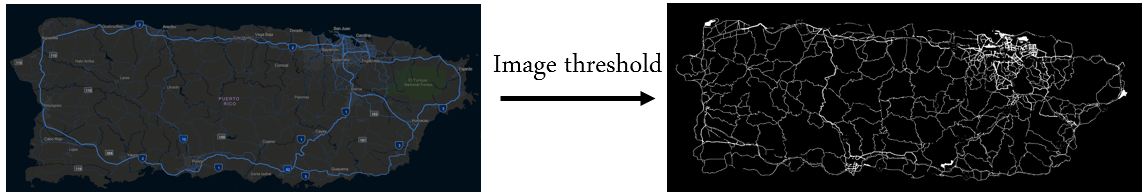
\includegraphics[scale=0.6]{threshold.png}
        \caption{Shows the result after threshold.}
    \end{figure}
\subsubsection{Dilated The Image} 
    We dialte the image (using $8 * 8$ Convolution kernel).On the one hand, the new white area represents the area that our drone can detect, on the other hand, 
    this can be our better plan for the reconnaissance trajectory and delivery route of the medicine.
    
    \centerline{Convolution Kernel $=\left[\begin{array}{cccccccc}{1} & {1} & {1} & {1} & {1} & {1} & {1} & {1} \\ {1} & {1} & {1} & {1} & {1} & {1} & {1} & {1} \\ {1} & {1} & {1} & {1} & {1} & {1} & {1} & {1} \\ {1} & {1} & {1} & {1} & {1} & {1} & {1} & {1} \\ {1} & {1} & {1} & {1} & {1} & {1} & {1} & {1} \\ {1} & {1} & {1} & {1} & {1} & {1} & {1} & {1} \\ {1} & {1} & {1} & {1} & {1} & {1} & {1} & {1} \\ {1} & {1} & {1} & {1} & {1} & {1} & {1} & {1} \\ {1} & {1} & {1} & {1} & {1} & {1} & {1} & {1}\end{array}\right]$}

    \lstset {language=C++}
        \begin{lstlisting}
            cv::Mat element = cv::getStructuringElement(cv::MORPH_RECT, cv::Size(8, 8));
            cv::dilate(out, out_dilated, element);
    \end{lstlisting}

    
    \begin{figure}[h]
        \centering
            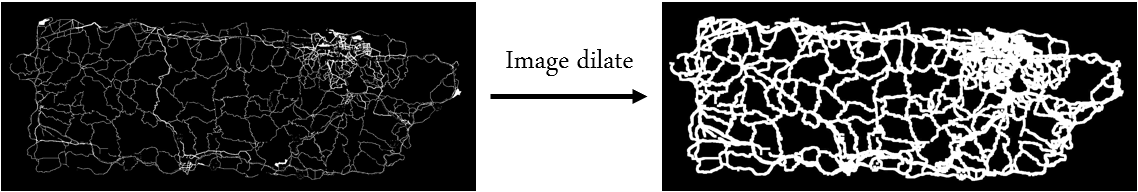
\includegraphics[scale=0.6]{dilate.png}
        \caption{Shows the result after dilated.}
    \end{figure}

\subsubsection{Detct And Extract The Cities Location}
By performing image feature detection and circle fitting, 
we can extract the locations of various cities for later road reconnaissance.
    \lstset {language=C++}
    \begin{lstlisting}
        medianBlur(src, cimg, 5);
        GaussianBlur(cimg, cimg, Size(9, 9), 2, 2);
        Canny(cimg, cimg, 10, 250, 5);
        vector<vector<Point>>cnts;
        findContours(cimg, cnts, RETR_EXTERNAL, CHAIN_APPROX_NONE);
        for (int i = 0; i < cnts.size(); i++)
        {
            vector<Point> cnts_single = cnts[i];
            if (cnts_single.size() > 0)
            {
                vector<Point> approx;
                string shape = detect(cnts_single, approx);
                Moments M = moments(cnts_single);
                int cX, cY;
                if (M.m10 != 0)
                {
                    cX = int((M.m10 / M.m00));
                    cY = int((M.m01 / M.m00));
                }
                putText(cimg, IntToStr(cX) + " , " + IntToStr(cY), Point(cX, cY),
                 FONT_HERSHEY_SIMPLEX, 0.5, Scalar(255, 0, 255), 1);  
            }
        }
    \end{lstlisting}

    \begin{figure}[h]
        \centering
            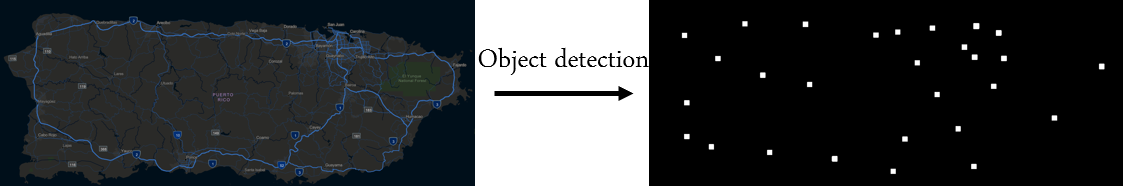
\includegraphics[scale=0.6]{object_detection.png}
        \caption{Shows the result after object detection.}
    \end{figure}

\section[]{Drone Flight Plan}
\subsection{Path Planning}





\end{document}


